\begin{figure}[h]
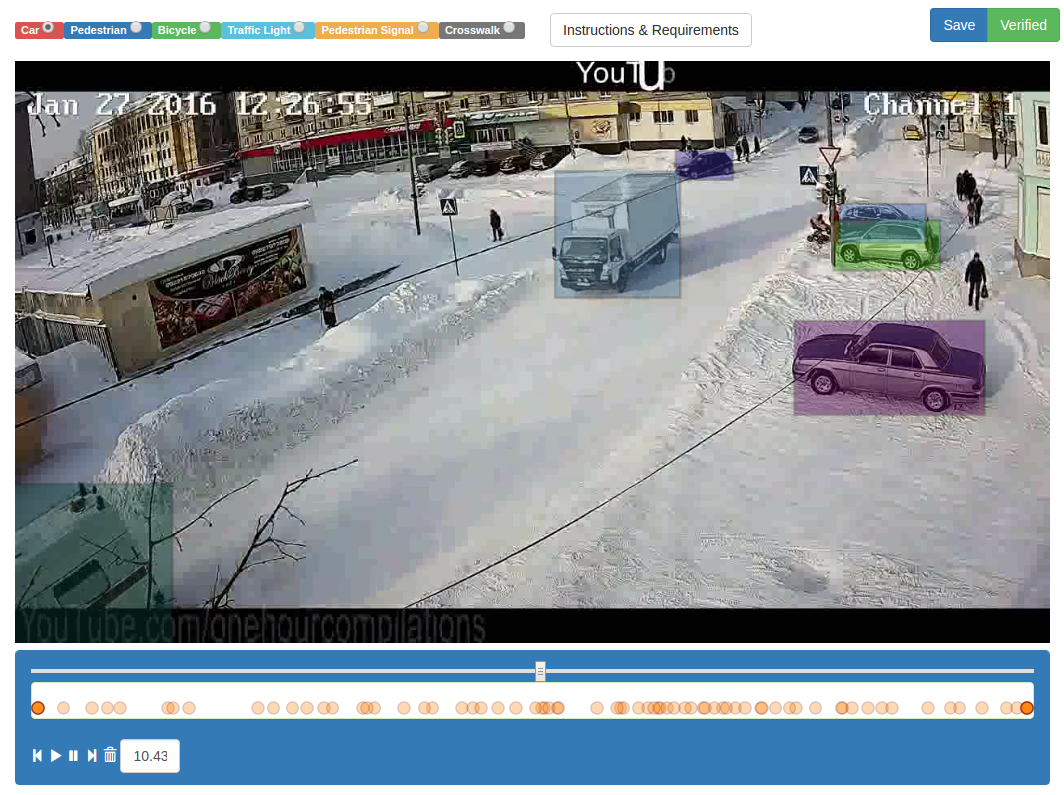
\includegraphics[width=15cm]{figs/interface.png}
\label{interface}
\centering
\caption{BeaverDam's expert verification interface with user keyframe scheduling enabled, border buffer disabled. Workers see a similar interface. Note the keyframe scheduling interface integrated with the video player, the single click multiple create interface, and objects being allowed to move partially or wholly off-screen in the bottom left corner.}
\end{figure}

The productivity of annotators is the focus of most of the prior works in this area.
During the development and deployment of BeaverDam, we've gathered extensive feedback from our turkers and testers.
We also implemented features suggested by past works such as VATIC,
and introduced several new ones to address issues found during the testing of VATIC.\footnote{Sceenshots of select issues in this chapter are taken from the demo video on VATIC's website, and are representative of what we encountered.}


\section{Keyframe scheduling}

A big decision for a keyframe-based video annotation tool is whether the worker or the tool chooses the keyframe schedule.
From past user studies, we know that human workers don't always choose the best keyframes, leading to inefficiencies.
In fact, VATIC showed that by switching to a fixed keyframe schedule, workers were able to label faster.
However, in our studies we found it to not always be the case.
Since our videos contain a varied mix of stationary objects, slow \& linearly moving objects, and fast objects with irregular motion, it makes sense to use fewer keyframes for easier objects.
While a flexible keyframe schedule could potentially be automated using tracking, we instead optimized the interface for user created keyframes.

We added a keyframe viewer bar that displays all keyframes and keyframes for the currently selected object.
The user can click on these keyframes to edit them, or insert new keyframes by editing the boxes when on a frame that's not a keyframe.
We also included keyboard shortcuts to jump between keyframes for experts who need finely grained editing.

\section{Video playback for maintaining identity}

VATIC's video player was a rudimentary image changer as its purpose was to give workers context when tracking objects.
As we wanted more flexibility and power for more advanced labelers, we incorporated a full fledged video player over VATIC's usage of JavaScript to advance images of frames.

One huge issue we solved with this setup was video loading times.
When deploying VATIC, we found users complaining about load times, and sometimes jobs would time out before the video loaded, especially when using high resolution images for frames.
When seeking in the video, the images would flash to white if it's not loaded from cache quickly enough. The interruption causes not only context loss but also frustration.
By converting the app to use HTML5 video, we take advantage of the ability to stream, similar to how YouTube and other sites can display video without loading all of it first.
The annotator can then begin annotating as the video loads.
The playback is also much smoother, with a minor tradeoff of slightly slower rewinds, as videos are encoded in a way optimized for forward playback. # something about studies where VATIC users used forward playback more often than rewinds would be good here

\section{Reducing clicks}

In addition to measuring the time it takes for annotators to perform certain actions, we sought to minimize the number of clicks necessary.
We find this to be a good rule of thumb when we don't have enough users to properly A/B test design choices.

First, we set the user in the hybrid create/edit mode by default.
A new object is created if the user drags in an empty spot, and an existing object is edited otherwise.
VATIC requires the user to click a ``create'' button, which enables the user to annotate heavily overlapped objects more easily.
We propose that it's more efficient to force a user to perform the extra steps of creating a box in an empty spot and dragging it onto the object in case of overlap,
as heavy overlaps turned out to be rare in our datasets, so it was better to optimize for the common case. # Woot its like Huffman, optimize for freq :D

\begin{figure}[h]
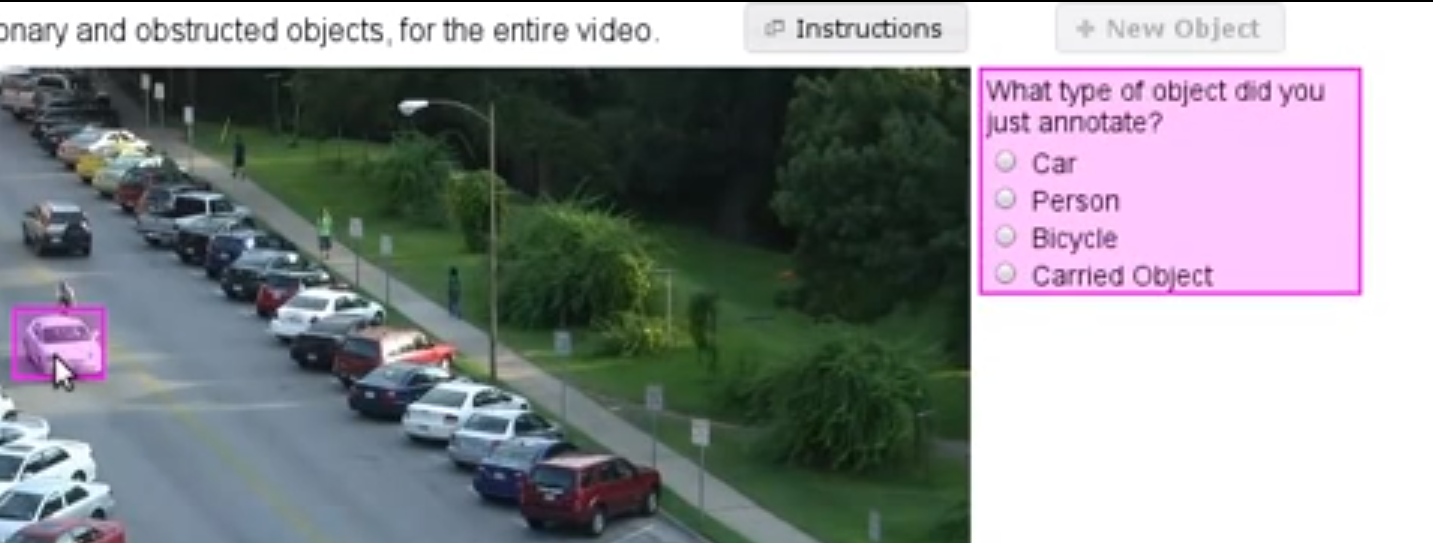
\includegraphics[width=14cm]{figs/vatic_create.png}
\centering
\caption{Explicit object creation in VATIC. BeaverDam guesses whether the worker wants to create a new object or edit an existing one by where they click, which is efficient in the general case. We also eliminate this additional prompt of asking for the object type and assume the type is same as the last created type by default.}
\end{figure}

Additionally, instead of having the user choose the type of object each time, we default to the most common label (car) or the user's last selection.
This reduced clicks, but did result in more errors for new users who didn't notice that they must change the label from the default when labeling non-cars.
While VATIC's prompting each time prevented this, we elected to solve it through a better tutorial to save time for acclimated annotators.

Finally, BeaverDam includes extensive keyboard shortcuts, with the aim of eliminating any need for the mouse aside from drawing and moving boxes.
Tasks such as label selections and video playback are all controlled through the keyboard.
We left in optional mouse controls, but it may be a good choice to remove them to enforce the faster keyboard workflow.
Surprisingly, we have had turkers report that they were on tablets, and keyboard shortcuts were inefficient for them.
However, we find in our small sample of annotators that tablet users are few, and less efficient in general.

\section{Handling frame exit/enters}

During our user tests, we found that users have the most difficulty when objects are entering or exiting the frame, as it's difficult for linear interpolation to handle a box whose size is increasing but one edge is fixed to the edge of the frame.

\begin{figure}[h]
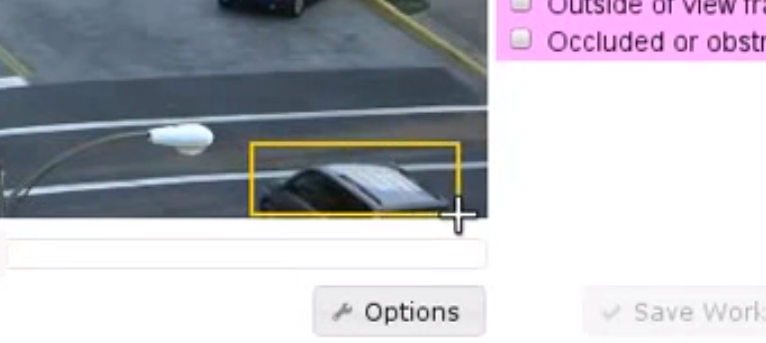
\includegraphics[width=14cm]{figs/vatic_border.png}
\centering
\caption{VATIC annotation of object entering frame. Note the user must draw the box exactly to the edge of the screen as shown here, as drawing fails otherwise. BeaverDam allows the user's mouse to draw to outside the frame, cropping back to the frame edge in post processing.}
\end{figure}

This was one of the main challenges when annotating using VATIC, as we had many driving videos where objects frequently entered and exited.
To address this issue, we introduced two solutions.
First, we allow boxes to be partially or wholly located outside the frame.
This enables the user to guess at the true location of the object if the frame were bigger, which allows for much better linear interpolation. % TODO: EXAMPLE OF THIS
Then, we add a large padding around the border of the frame, essentially enlarging the frame with blank space, which makes drawing and editing boxes that are located partially outside the frame much easier.
After labeling, any boxes that are partially outside the frame can be cropped to the edge of the frame.


% \section{Micro vs Macro tasks}

% The topic of whether to divide up work to give each worker a small task to be completed in less than a minute (micro task) has been well discussed in literature.
% In ImageNet and other image classification \& detection datasets, micro tasks were preferred as they provided the workers more predictable task completion times and reward schedules.
% They are also easier for quality control as gold standard tasks where the label in known can be dispersed among the tasks.
% However, the authors of VATIC found through their experiments that macro tasks were better for video annotation, as errors from earlier tasks propagated throughout the rest of the video.
% We compared these two competing philosophies of expert annotators completing large tasks vs using many independent small tasks.



% Comparison from existing literature

% Proposal advocating for micro-tasks in video labeling

% Extensible task structure

% \section{Interpolation \& Tracking}

